\documentclass[tikz, border=10pt]{standalone}
\usetikzlibrary{arrows.meta, positioning, shapes, calc}

\usepackage[T1]{fontenc}
\usepackage{lmodern}
\begin{document}
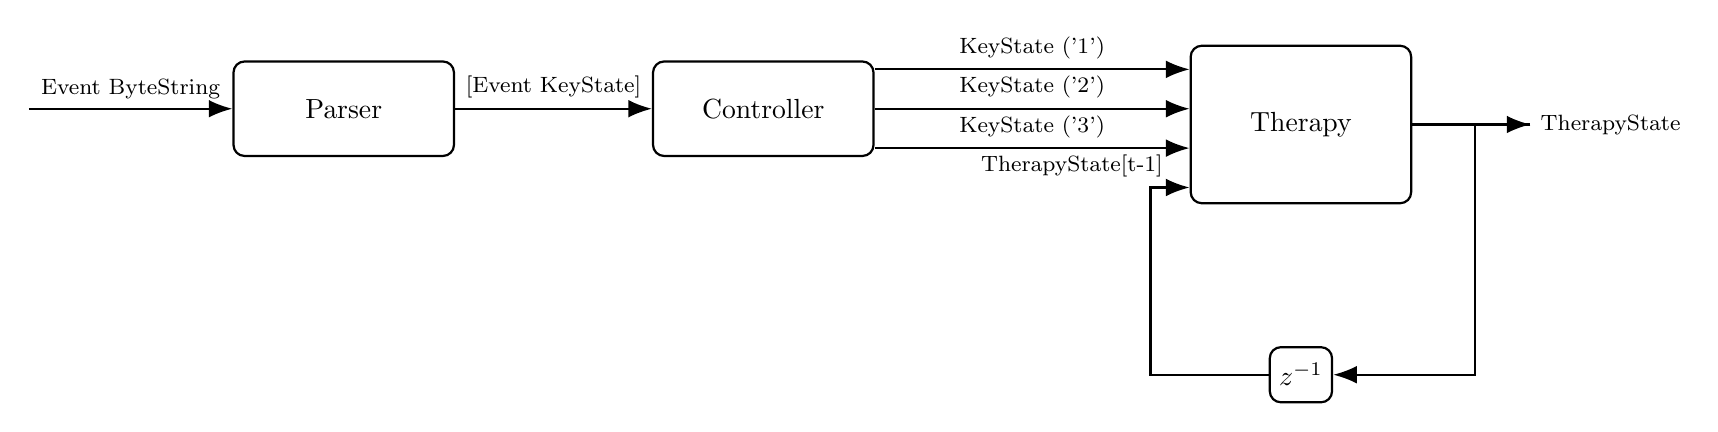
\begin{tikzpicture}[
  block/.style = {draw, thick, minimum width=2.8cm, minimum height=1.2cm, align=center, rounded corners},
  sum/.style = {draw, circle, inner sep=1pt, minimum size=6mm, node contents={+}},
  line/.style = {thick, -{Latex[length=3mm]}},
  signal/.style = {font=\footnotesize, midway, above},
  signalbelow/.style = {font=\footnotesize, midway, below}
]

% Nodes
\node[block] (parser) {Parser};
\node[block, right=2.5cm of parser] (controller) {Controller};
\node[block, right=4cm of controller, minimum height=2.0cm, yshift=-0.2cm] (therapy) {Therapy};
  \node[block, minimum size=7mm, below=1.8cm of therapy] (delay) {$z^{-1}$};

% Connections
\draw[line] (-4,0) -- (parser.west) node[signal]{Event ByteString};
\draw[line] (parser.east) -- node[signal]{[Event KeyState]} (controller.west);

% Controller to Therapy lines
\foreach \y/\label in {0.7/{KeyState ('1')}, 0.2/{KeyState ('2')}, -0.3/{KeyState ('3')}} {
  \draw[line] ([yshift=\y cm - 0.2cm]controller.east) -- node[signal]{\label} ([yshift=\y cm]therapy.west);
}

% Therapy output
\draw[line] (therapy.east) -- ++(1.5,0) coordinate (out) node[right, font=\footnotesize]{TherapyState};

% Feedback path through delay
\draw[line] (out) -- ++(-0.7,0)|- (delay.east);
  \draw[line] (delay.west) -| ++(-1.5,1.8) |- ([yshift=-0.8cm]therapy.west) node[signal, above, xshift=-1cm]{TherapyState[t-1]};

\end{tikzpicture}
\end{document}
